\documentclass[10pt,aspectratio=43]{beamer}

\usepackage{graphicx}
\usepackage{tikz}
\usepackage{xcolor}
\usepackage{caption}
\usepackage{subcaption}
\usepackage{bm}
\usetikzlibrary{calc} 
\usepackage{hyperref}
\hypersetup{
    colorlinks=true,
    linkcolor=blue,
    urlcolor=red
}
\usepackage{fontawesome5}
\usepackage{ulem}
\usepackage[dvipsnames]{xcolor}

\usetheme{MyStyle}   % loads beamerthemeMyStyle.sty
\setlength{\columnsep}{0pt}


%%%%%%%%%%%%%%%%%%%%%%%%%%%%%%%%%%%%%%%%%%
%%%%%%%%%%%%%%%%%%%%%%%%%%%%%%%%%%%%%%%%%%
%%%%%%%%%%%%%%%%%%%%%%%%%%%%%%%%%%%%%%%%%%

\title{Rapport de 2ème année de doctorat}
\newcommand{\eventname}{CSI meeting}
\author{Felix Touchte Codjo}
\institute{IJCLab}
%\date{\today}
\date{September 28, 2026}


\begin{document}

\begin{frame}[plain] % remove header, footer, barre de navigation
\titlepage
\end{frame}

%\begin{frame}{Outline}
%\tableofcontents
%\end{frame}

% \begin{frame}{Features of GPDs}
%     \begin{itemize}
%         \item Correlation between PDF and FF
%         \item 3D imaging in impact parameter space
%         \item Spin puzzle
%         \item Pressure and shear force
%     \end{itemize}

% \end{frame}


\begin{frame}{Nuclear GPDs}
    \begin{itemize}
        \item Access parton GPDs from the nucleus as a whole
        \item Compare to those obtained in free proton
        \item Reveal variety of nuclear effects
            \begin{itemize}
                \item e.g. modification of the quark confinement size
                \item e.G. short range correlation
            \end{itemize}
        \item Provide new insight into the understanding of the EMC effect
    \end{itemize}

\end{frame}


\begin{frame}{Nuclear GPD with A}
    \begin{itemize}
        \item Access quark GPD via DVCS
        \item In nuclear target : coherent DVCS and incoherent DVCS
        \item HERMES : first attempt but failed to distinguish coherent and incoherent events
        \item CLAS eg6 : first DVCS off He4, highlights the benefit of detecting the recoil nucleus
        \item ALERT : extend eg6 at 12 GeV to cover more phase space
    \end{itemize}

\end{frame}


% \begin{frame}{Experiment at JLab}
%     \begin{itemize}
%         \item CEBAF : 12 GeV polarized beam
%         \item CLAS12 : large acceptance detector help to cover large phase space
%         \item Need a new detector to achieve the physics program
%         \item The default setup can only detect $p > 250$ MeV/c in the central region
%         \item The previous RTPC
%             \begin{itemize}
%                 \item Limited PID capabilities for the detection of $^3\mbox{He}$ and $^3\mbox{H}$
%             \end{itemize}
        
%     \end{itemize}
    
% \end{frame}


\begin{frame}{ALERT detector}
    \begin{itemize}
        \item Technical requirements of the new detector
            \begin{itemize}
                \item Kinematics range: $70 < p < 400$ MeV/c, $\theta > 45^\circ$
                \item Replace the MVT and CVT located inside a 5T solenoid magnet
                \item Need to be transparent for the particle to be detected by CLAS
            \end{itemize}
        \item Solution ALERT = AHDC + ATOF
        \item The design makes ALERT fast and can be added in the trigger
    \end{itemize}
    
\end{frame}


\begin{frame}{ALERT run period}
    \begin{itemize}
        \item From April 2025 to September 2025
        \item Summary (HV, event rate, nominal beam current)
        \item Successful data taking
        \item Transition to the ongoing software development and data calibration
    \end{itemize}
    
\end{frame}


\begin{frame}{Overview of the ALERT reconstruction}

    \centering

    \begin{minipage}{0.45\textwidth}
        \begin{itemize}
            \item Decoding
                \begin{itemize}
                    \item From raw data to waveform
                    \item Waveform processing**
                \end{itemize}
            \item Hit selection
                \begin{itemize}
                    \item Waveform classification**
                    \item Selection cuts**
                \end{itemize}
            \item Track finder
                \begin{itemize}
                    \item MLP/GNN
                \end{itemize}
            \item Track fitting
                \begin{itemize}
                    \item Helix fitter
                    \item Kalman Filter*
                \end{itemize}
            \item Association AHDC track with ATOF hit
        \end{itemize}
    \end{minipage}
    \begin{minipage}{0.48\textwidth}
        \begin{itemize}
            \item Calibration
                \begin{itemize}
                    \item Time calibration
                    \item Time-to-distance calibration*
                \end{itemize}
            \item Alignment
                \begin{itemize}
                    \item Vertex alignment**
                    \item Phi alignment**
                    \item Beamline orientation
                \end{itemize}
        \end{itemize}
    \end{minipage}
    

\end{frame}


\begin{frame}{Pulse decoding}
    \begin{itemize}
        \item Information extracted from a signal
                \begin{itemize} \footnotesize
                    \item Baseline $\rightarrow$ estimated using the 4 first samples
                    \item Amplitude $\rightarrow$ after baseline subtraction, average of 3 samples around the peak
                    \item Leading edge time $\rightarrow$ computed at 1/2 amplitude
                    \item Time over threshold $\rightarrow$ computed if the signal has a trailing edge at 1/2 amplitude
                \end{itemize}
        \item The leading edge time is well determined for wfType 0 and 2
        \item However, the time reconstructed for saturated signals is underestimated using the previous method
                \begin{itemize} \footnotesize
                    \item Such bias will impact the reconstruction of $\alpha$ particle
                \end{itemize}
    \end{itemize}
    
    \vspace{0.3cm}
    \centering
    % 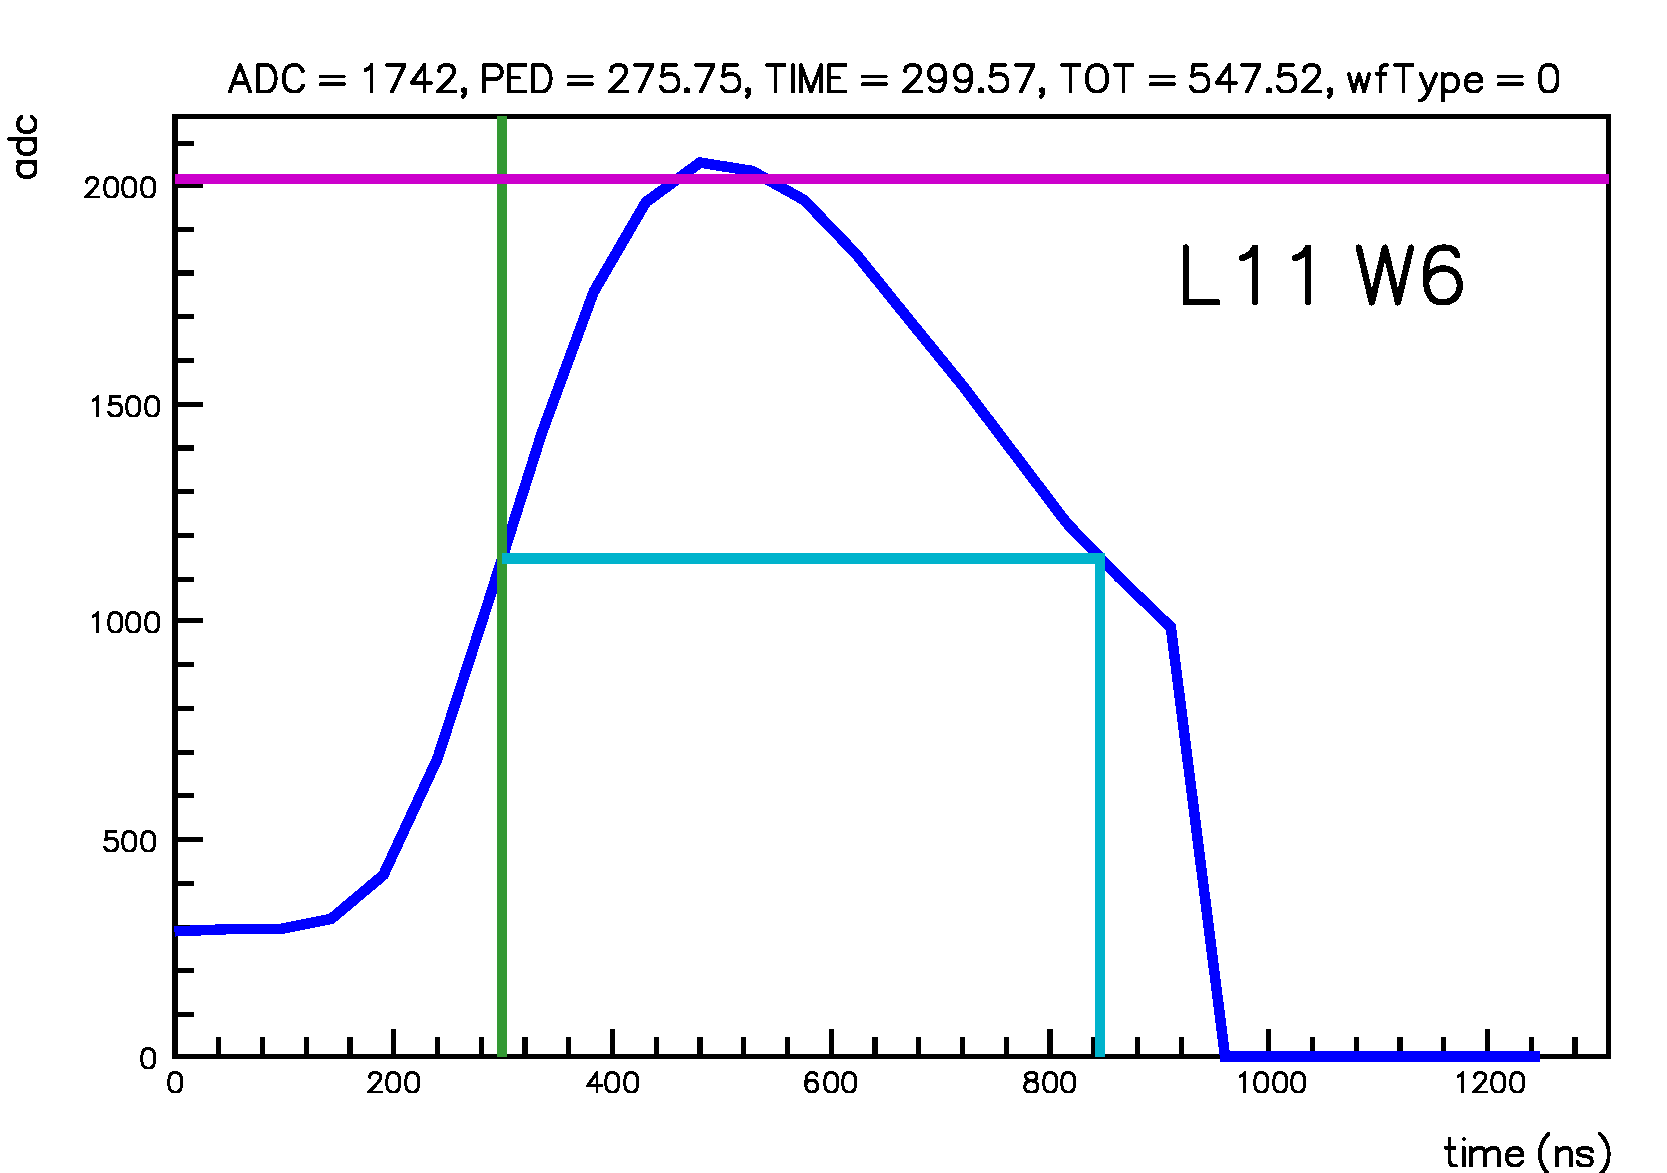
\includegraphics[width=0.4\linewidth]{figures/wf0_normal.pdf} 
    % \includegraphics[width=0.44\linewidth]{figures/build/adc_of_saturated_signals.pdf}

    \begin{minipage}{0.4\linewidth}
        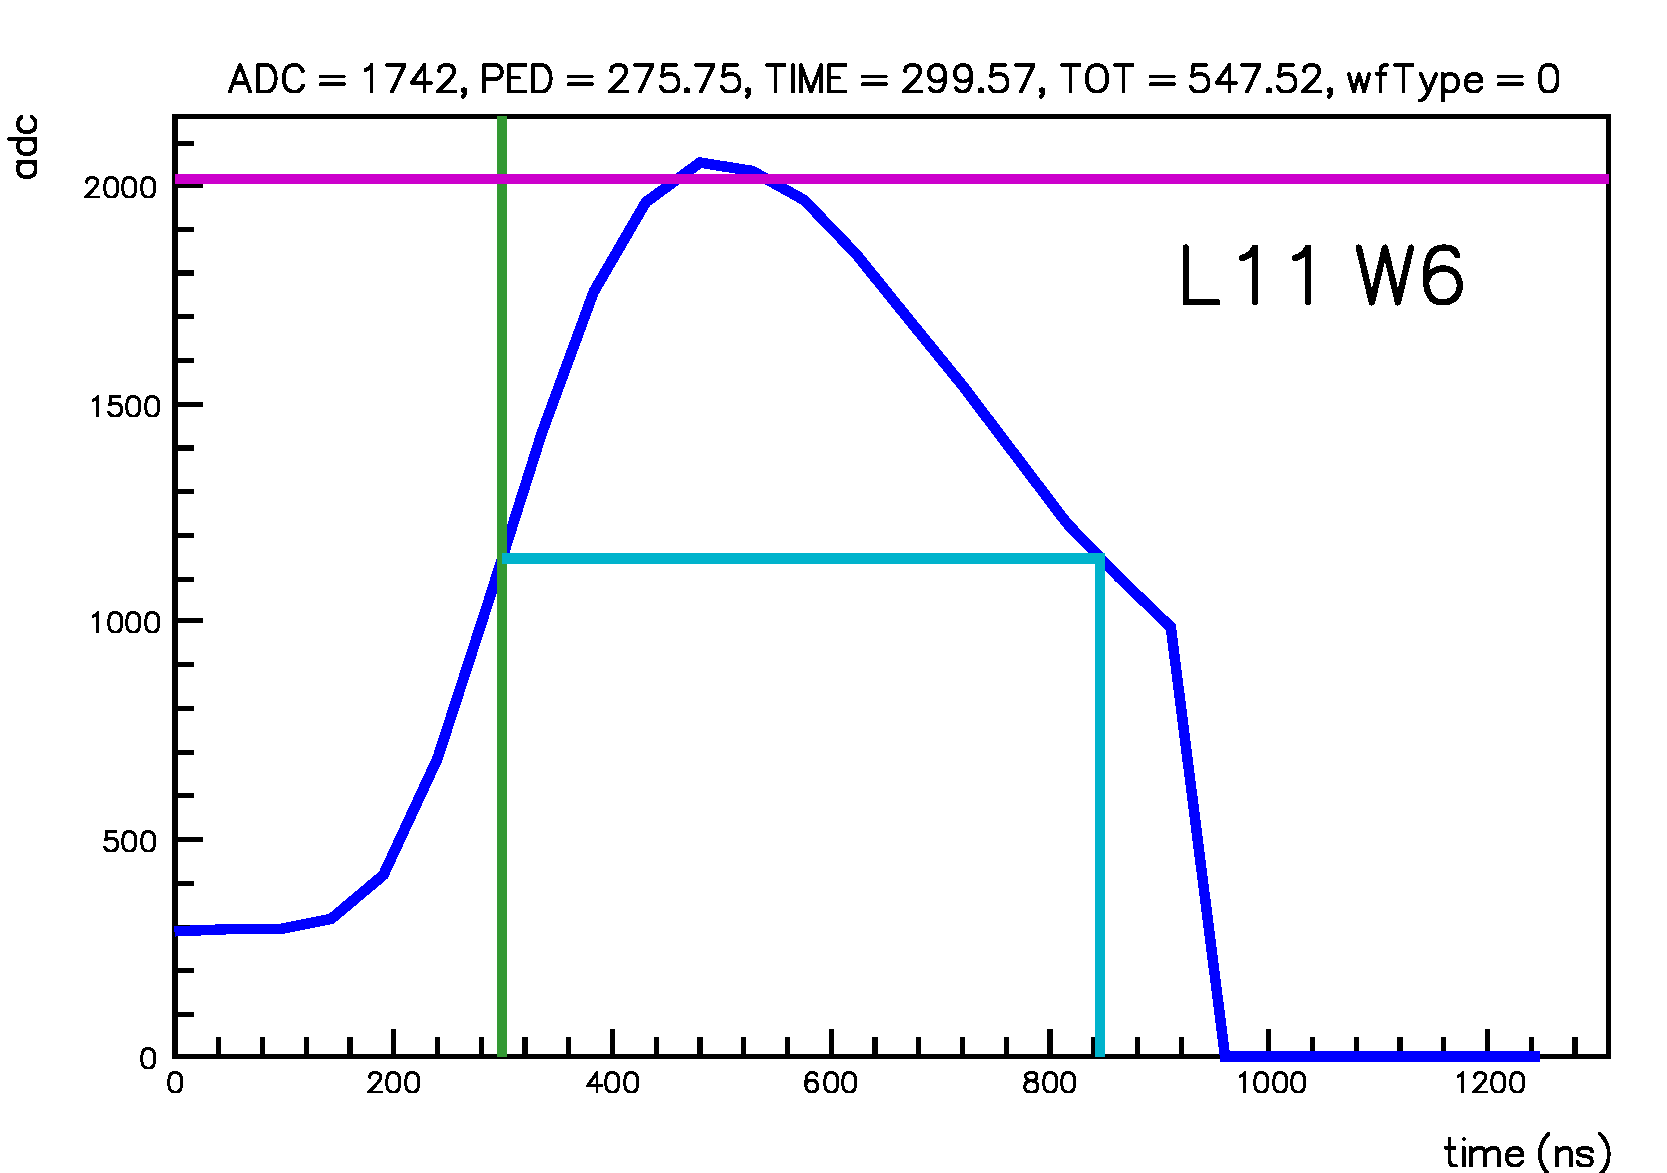
\includegraphics[width=\linewidth]{figures/wf0_normal.pdf} 
    \end{minipage}
    \begin{minipage}{0.42\linewidth}
        \includegraphics[width=\linewidth]{figures/build/adc_of_saturated_signals.pdf} 
    \end{minipage}

    
\end{frame}


\begin{frame}{Pulse decoding -- Saturated signals}

    \begin{minipage}{0.56\linewidth}
        \begin{itemize}
            \item The maximum of the slope of the signal is linearly correlated to the amplitude of non-saturated signals
                \begin{itemize}
                    \item We correct the amplitude of saturated signals using this trend
                \end{itemize}
            \item With the corrected amplitude, we recompute the time at 1/2 amplitude
        \end{itemize}
    \end{minipage}
    \begin{minipage}{0.4\linewidth}
        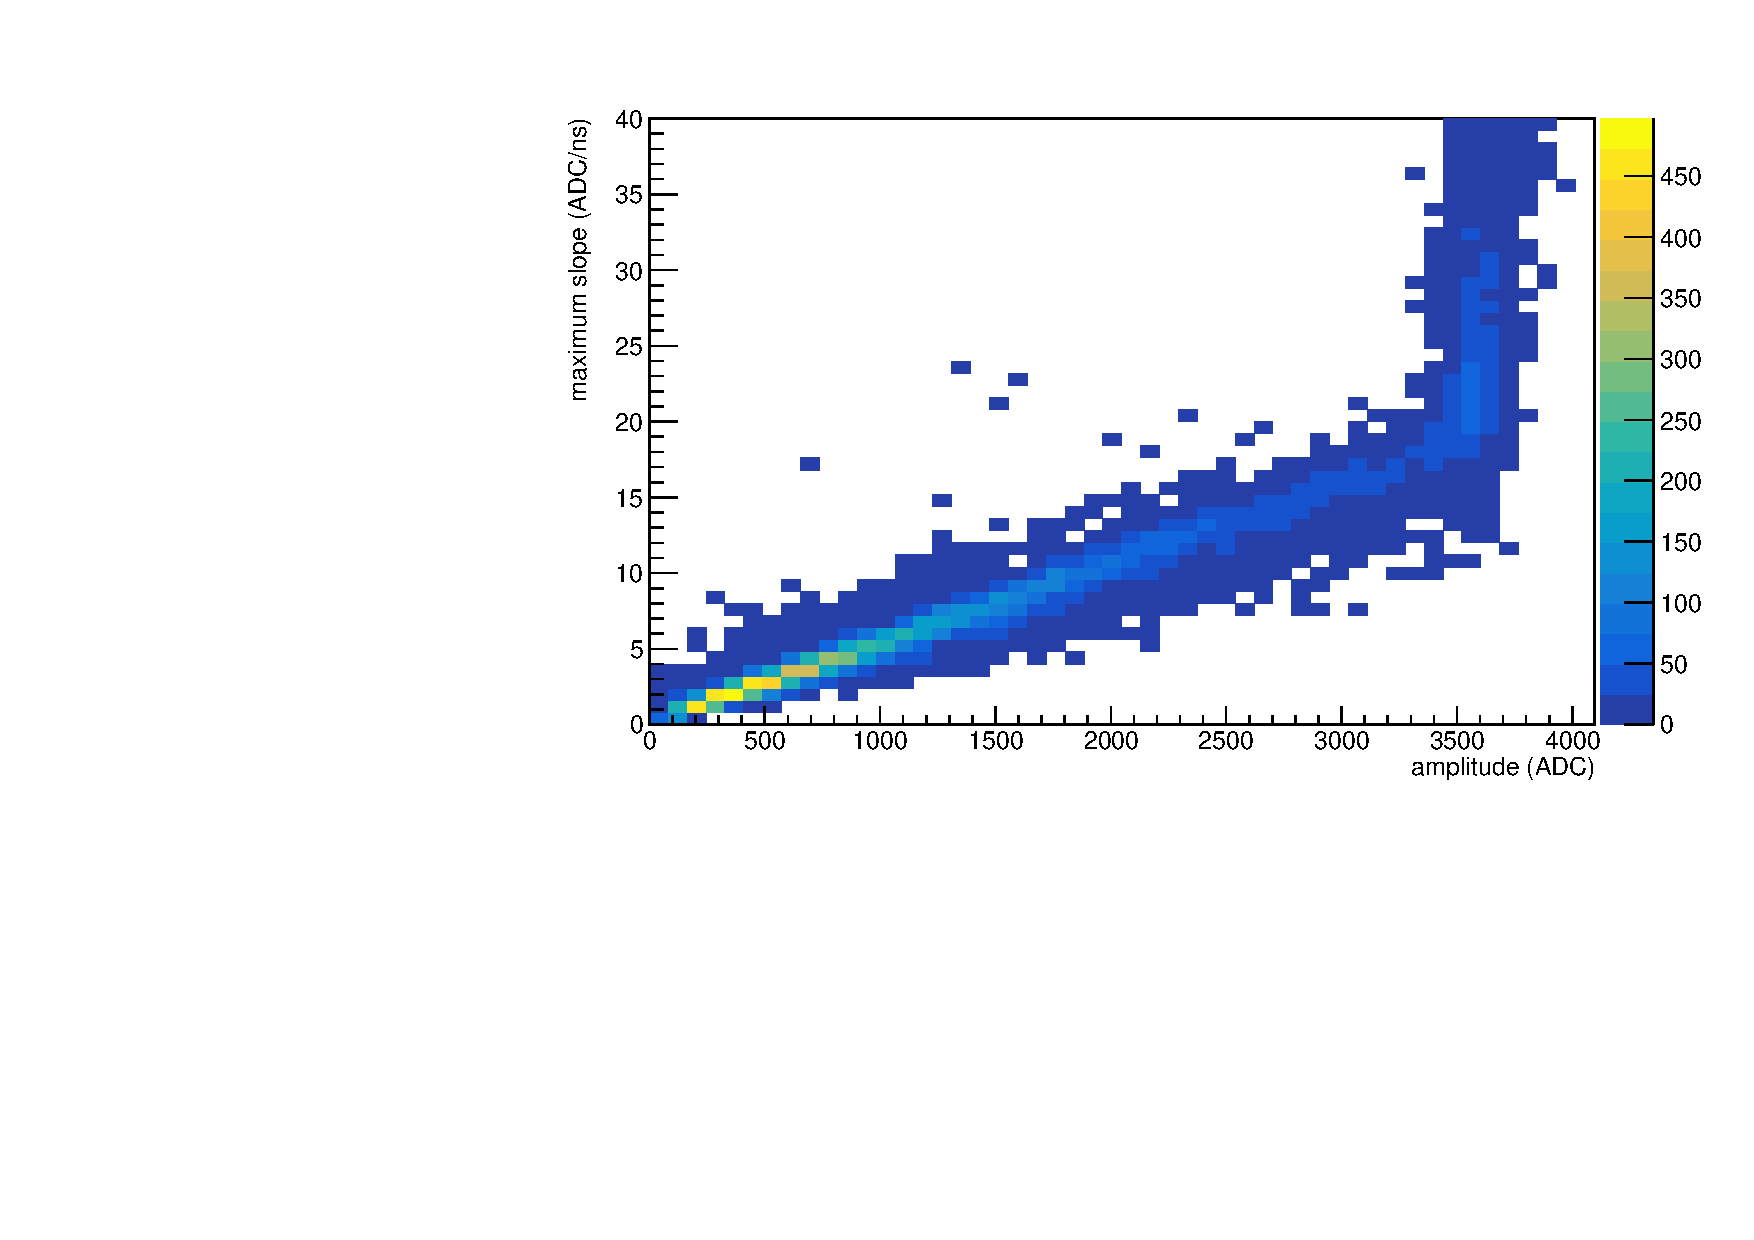
\includegraphics[width=\linewidth]{figures/slope_versus_adc_all_signals.pdf} 
    \end{minipage}

    \vspace{0.3cm}
    \centering    
    \begin{tabular}{cc}
        \includegraphics[width=0.4\linewidth]{figures/build/decoding_saturated_signals_normal.pdf} &
            \includegraphics[width=0.4\linewidth]{figures/build/decoding_saturated_signals_above_threshold.pdf} \\
        \footnotesize 1/2 ADC below threshold & 
            \footnotesize 1/2 ADC above threshold
    \end{tabular}
    
    
    
\end{frame}


\begin{frame}{Waveform classification}
    \begin{itemize}
        \item Noisy signals in AHDC have a repeated pattern
        \item Only signals with a good leading edge time are relevant (wfType $\leq$ 2)
    \end{itemize}

    \centering
    \vspace{0.3cm}
    {
        \footnotesize
        \begin{tabular}{l|l|l}
            wfType 6 $\rightarrow$ too short & wfType 5 $\rightarrow$ decreasing & wfType 4 $\rightarrow$ small ToT \\
            wfType 3 $\rightarrow$ pileup & wfType 2 $\rightarrow$ missing trailing edge & wfType 1 $\rightarrow$ saturated \\
            wfType 0 $\rightarrow$ normal & &
        \end{tabular}
    }

    \vspace{0.3cm}
    {
        \setlength{\tabcolsep}{1pt}
        \begin{tabular}{cccc}
            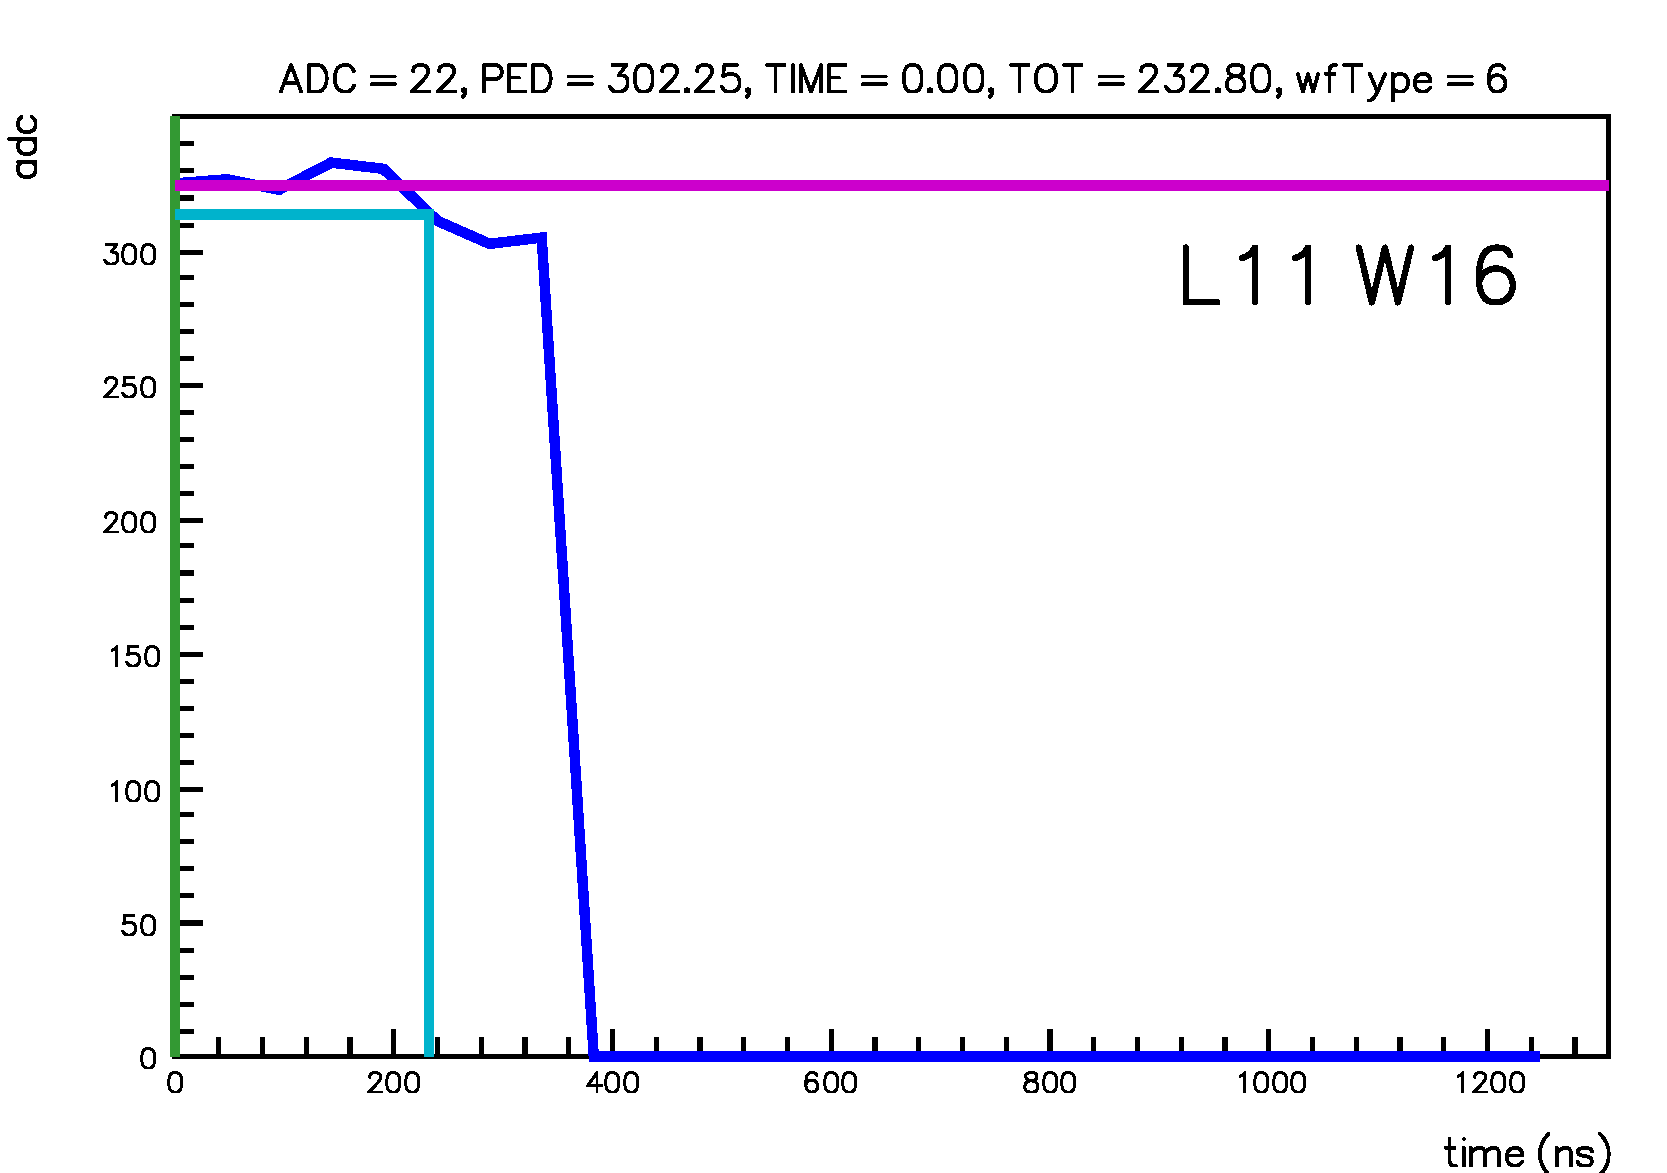
\includegraphics[width=0.24\linewidth]{figures/wf6_short.pdf} &
                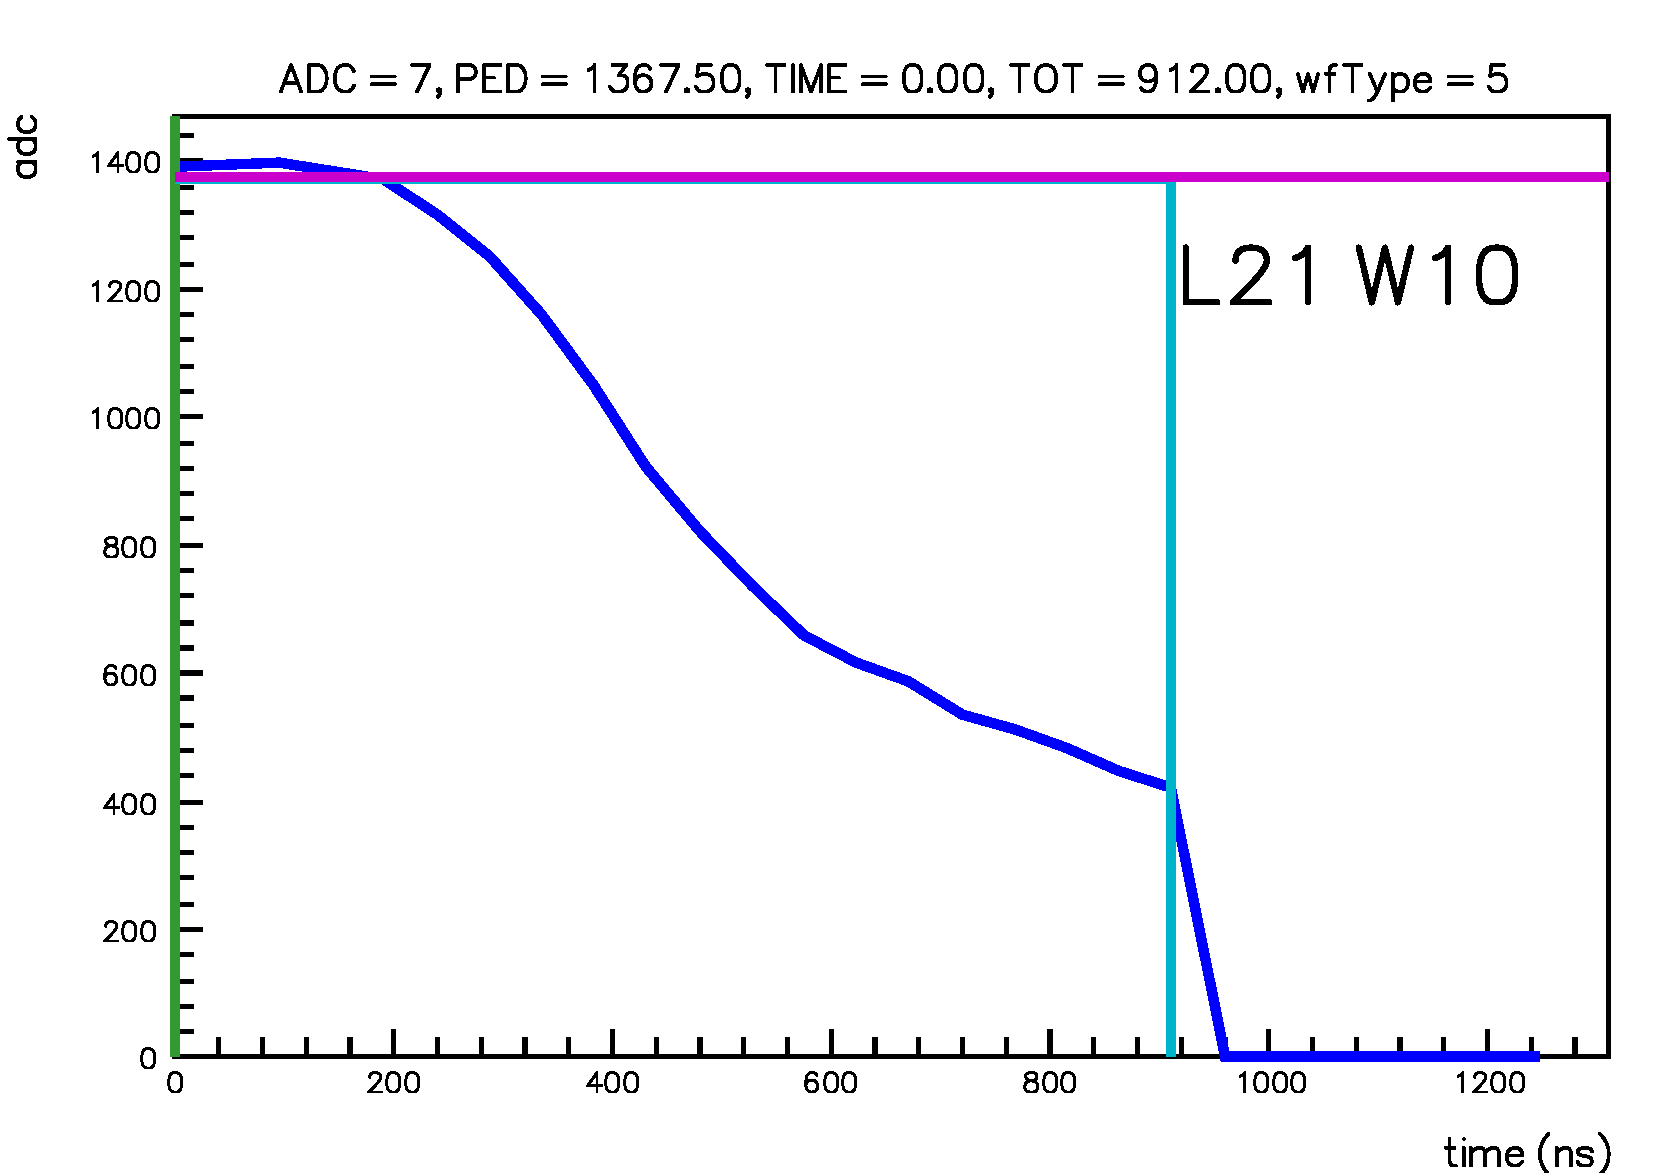
\includegraphics[width=0.24\linewidth]{figures/wf5_decreasing.pdf} &
                    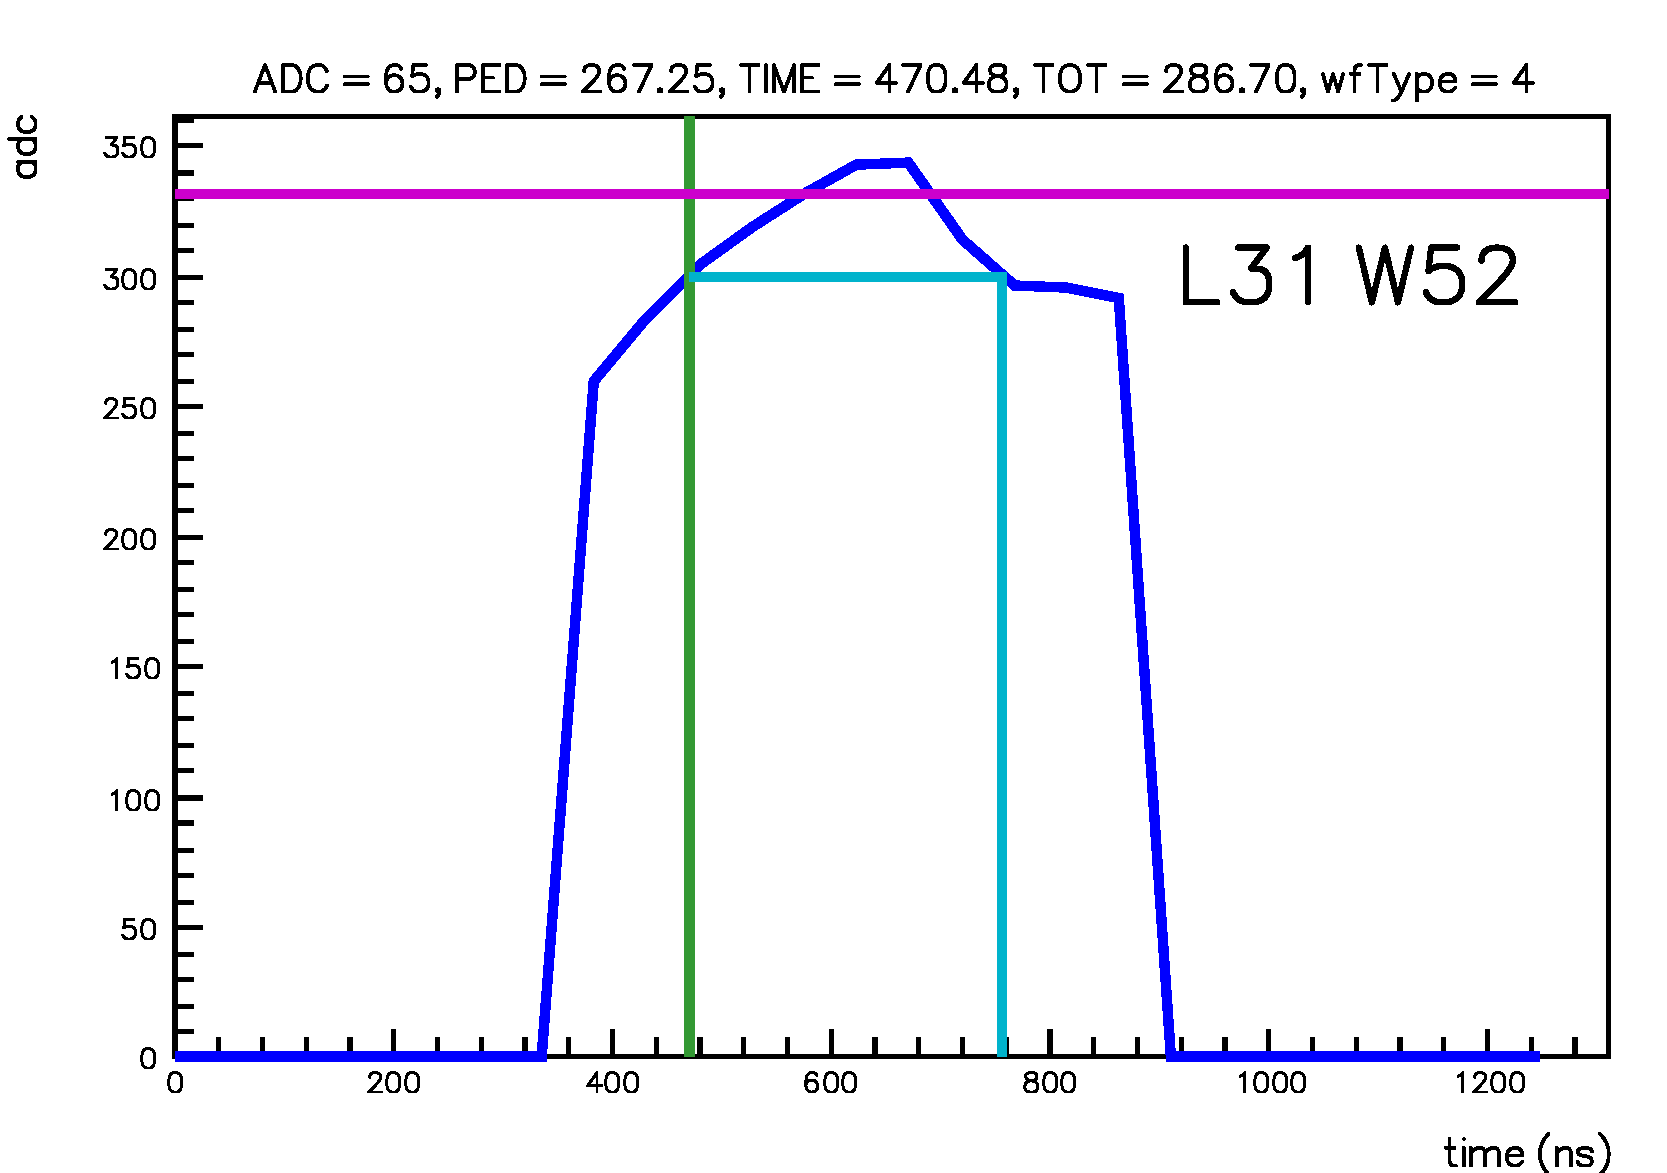
\includegraphics[width=0.24\linewidth]{figures/wf4_bad_tot.pdf} & 
                        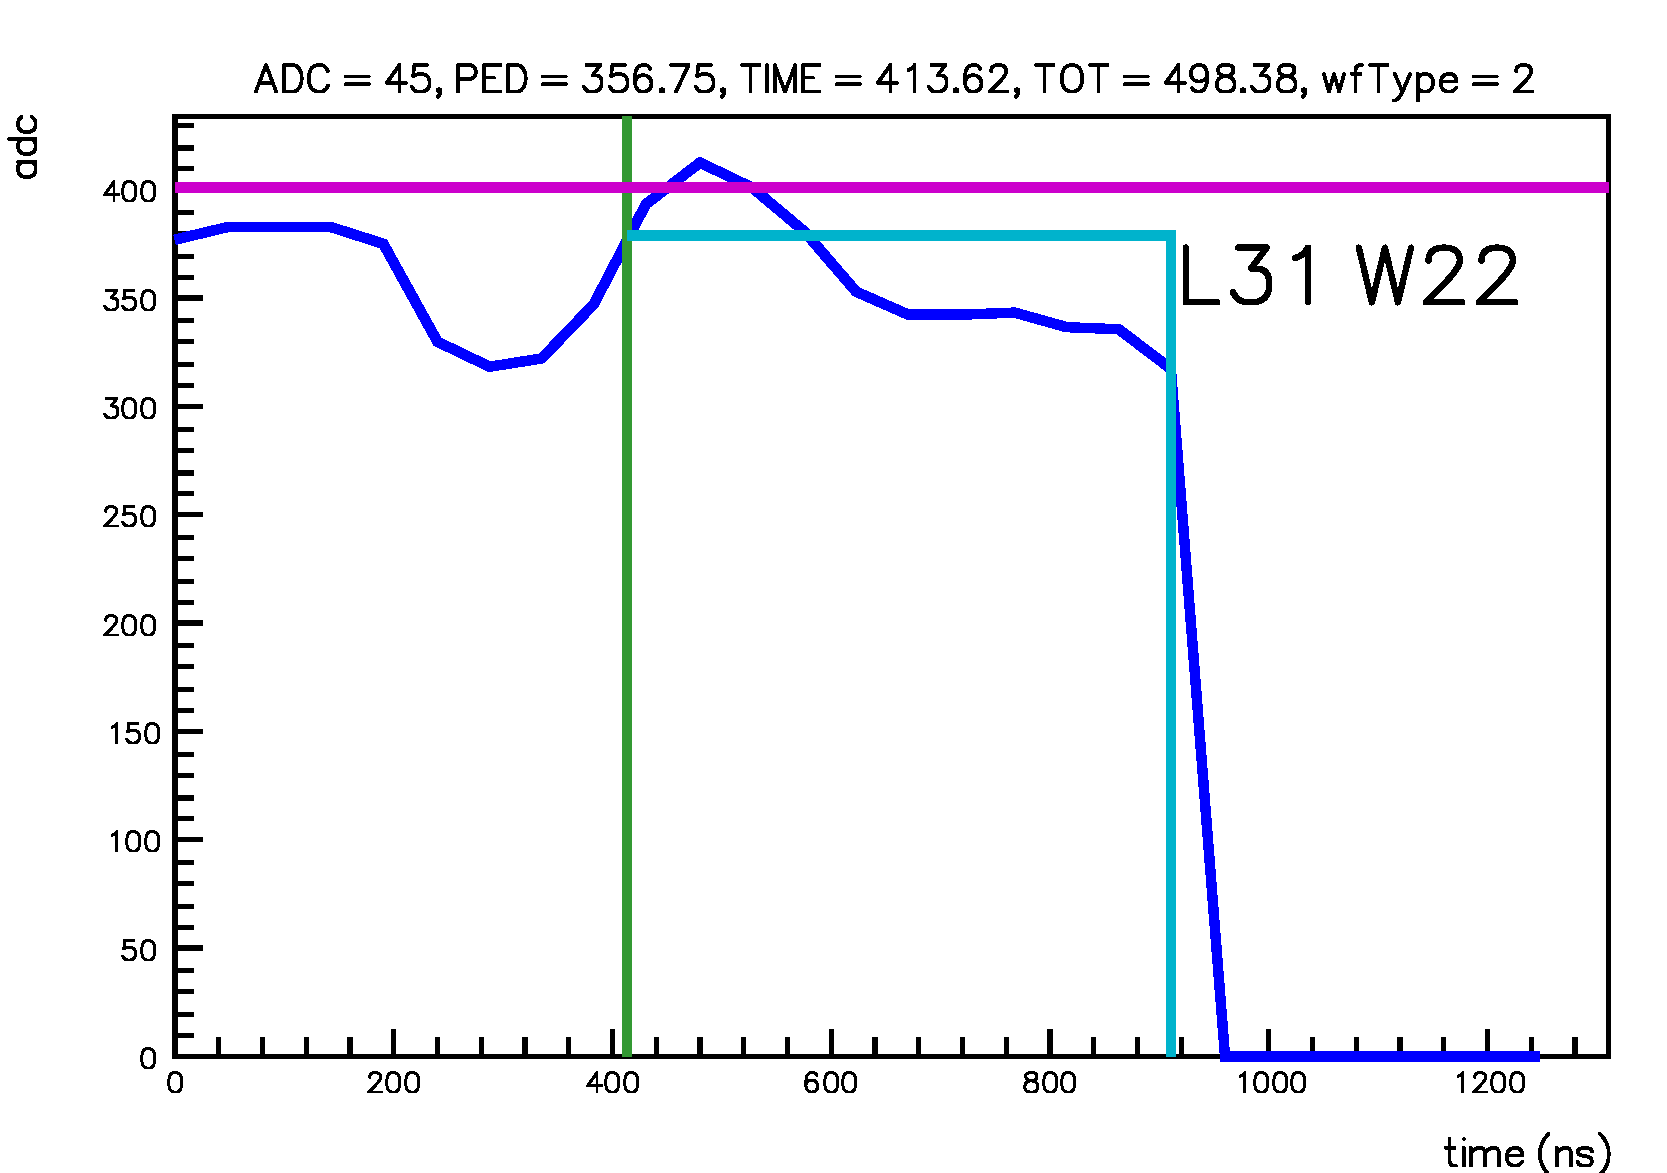
\includegraphics[width=0.24\linewidth]{figures/wf3_pileup.pdf} \\
            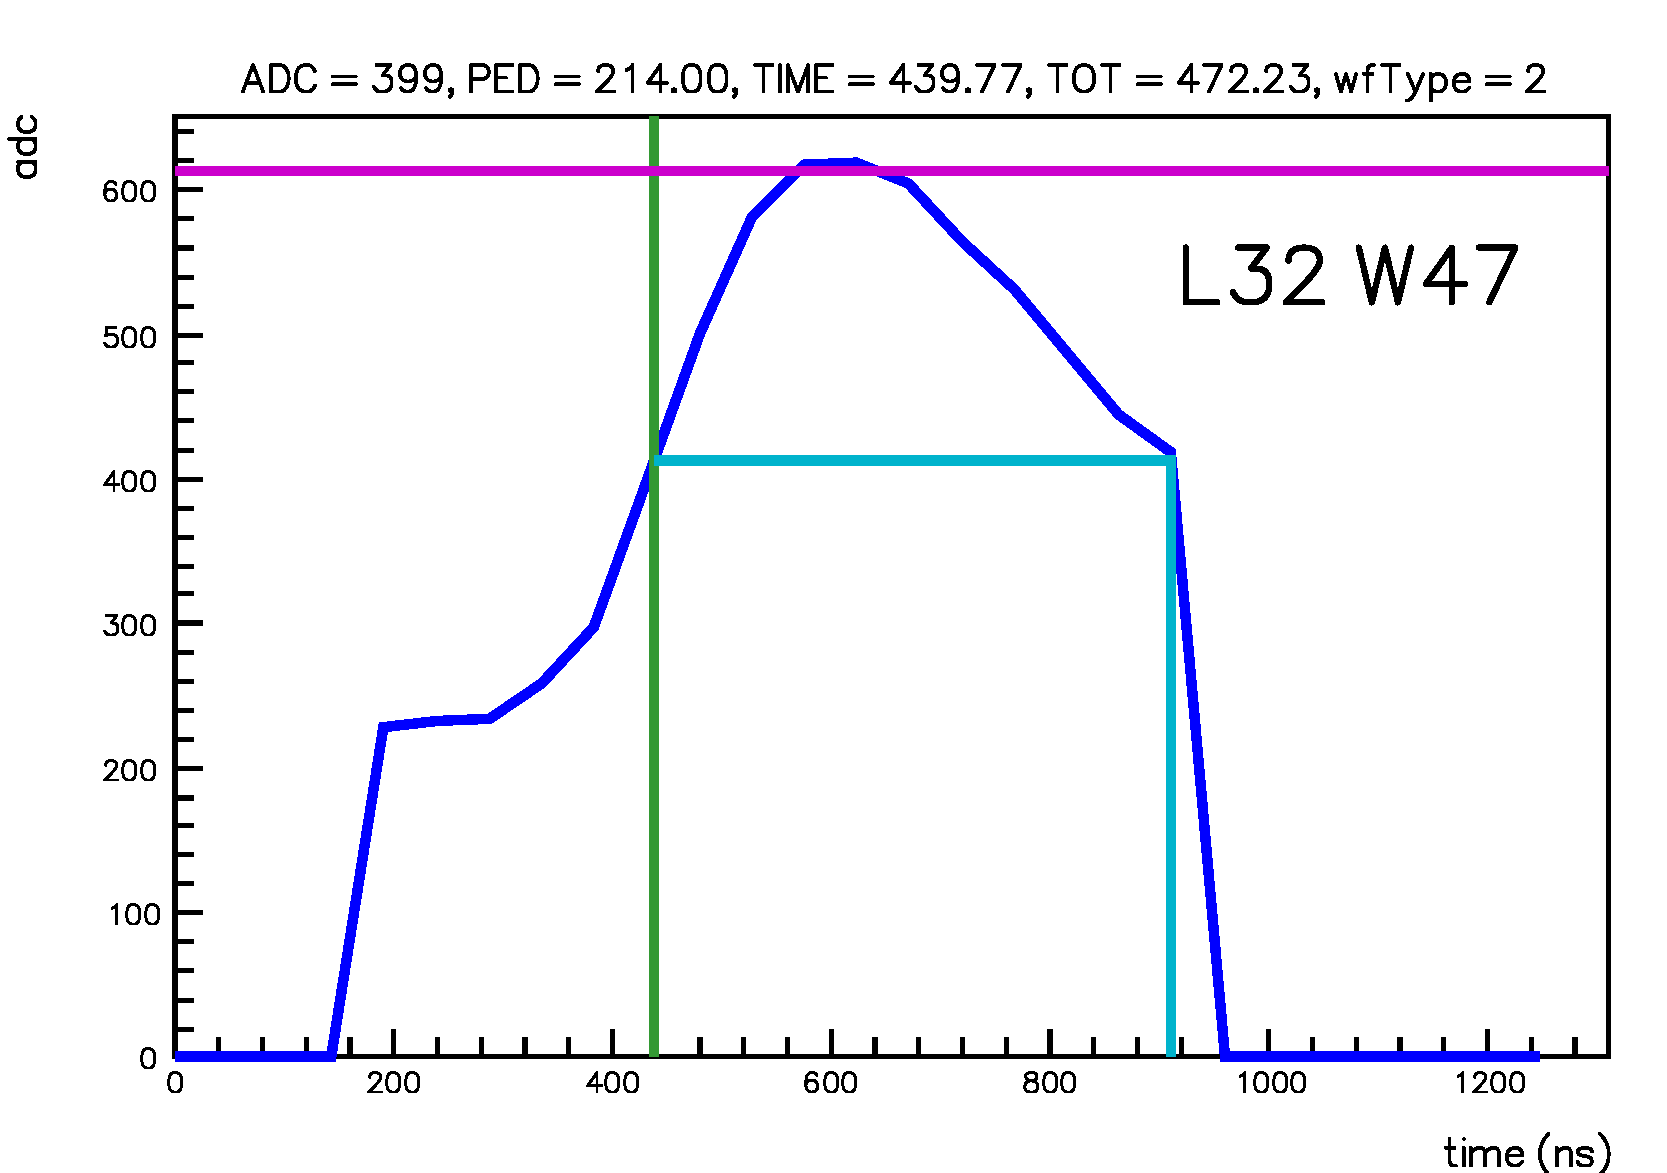
\includegraphics[width=0.24\linewidth]{figures/wf2_bad_trailing_edge.pdf} &
                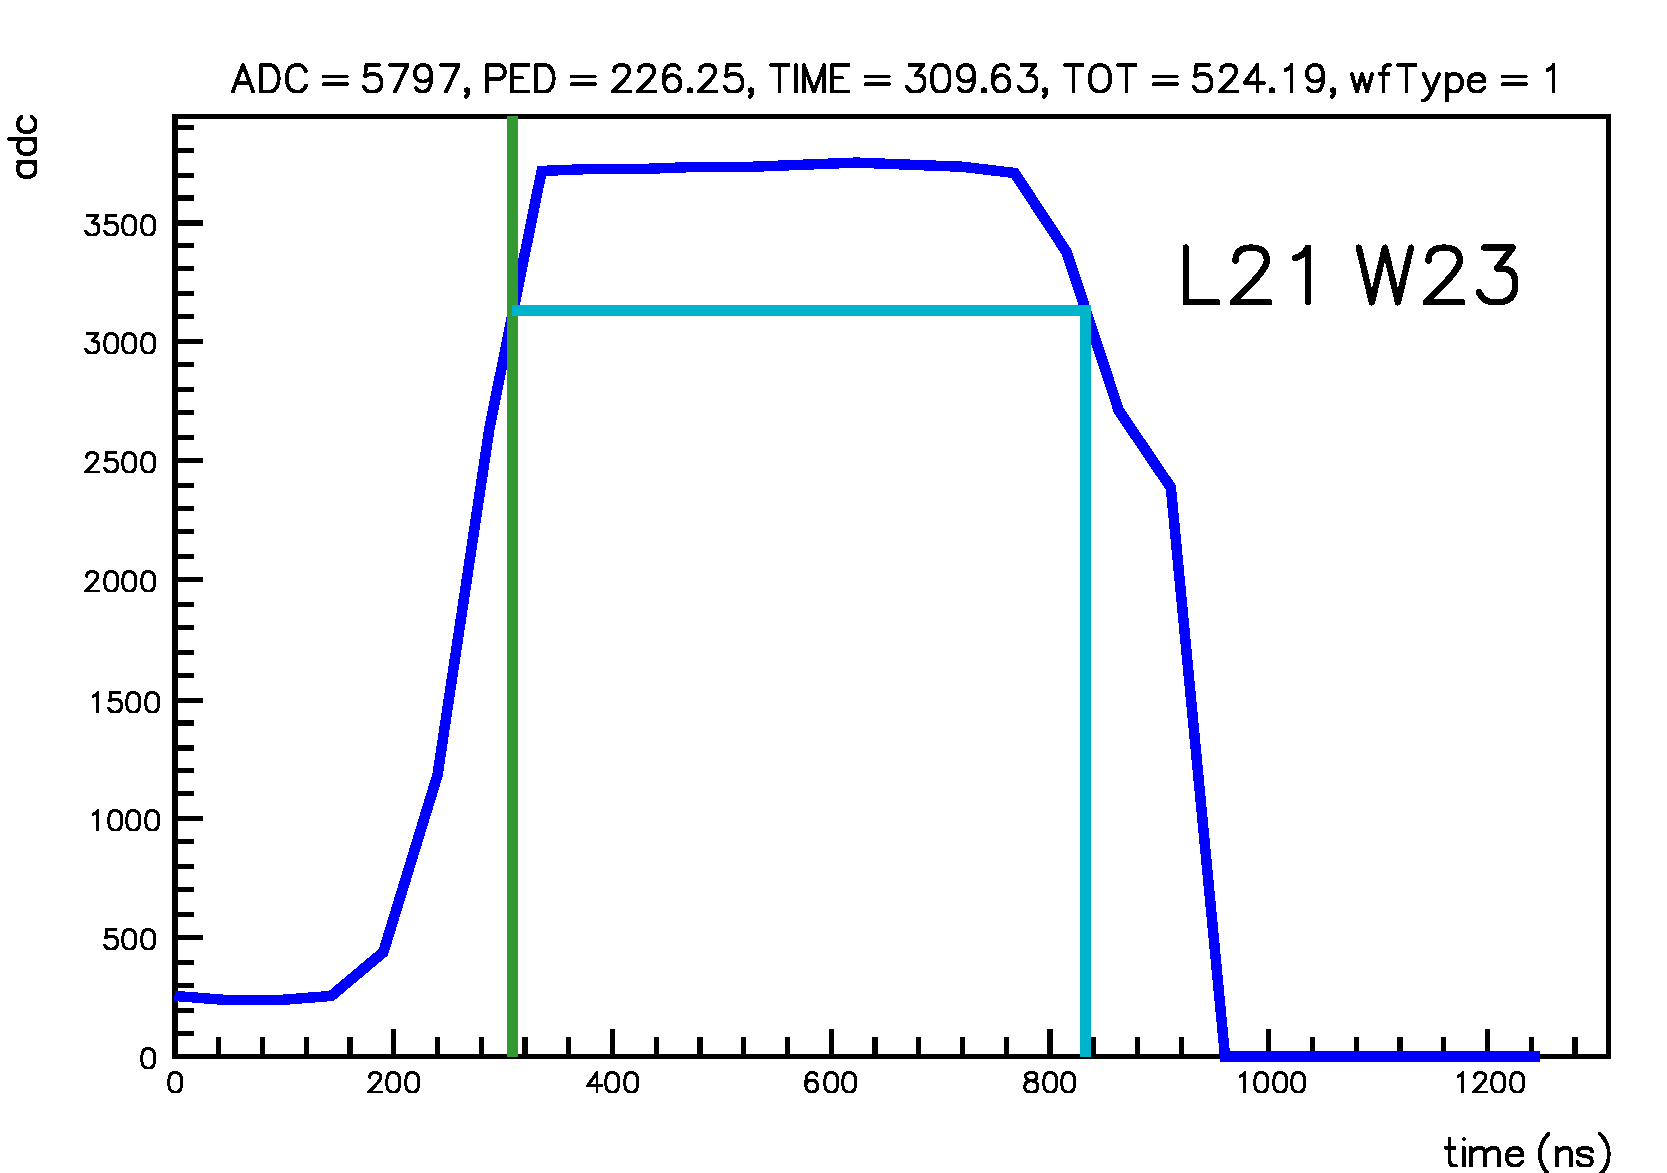
\includegraphics[width=0.24\linewidth]{figures/wf1_saturated.pdf} &
                    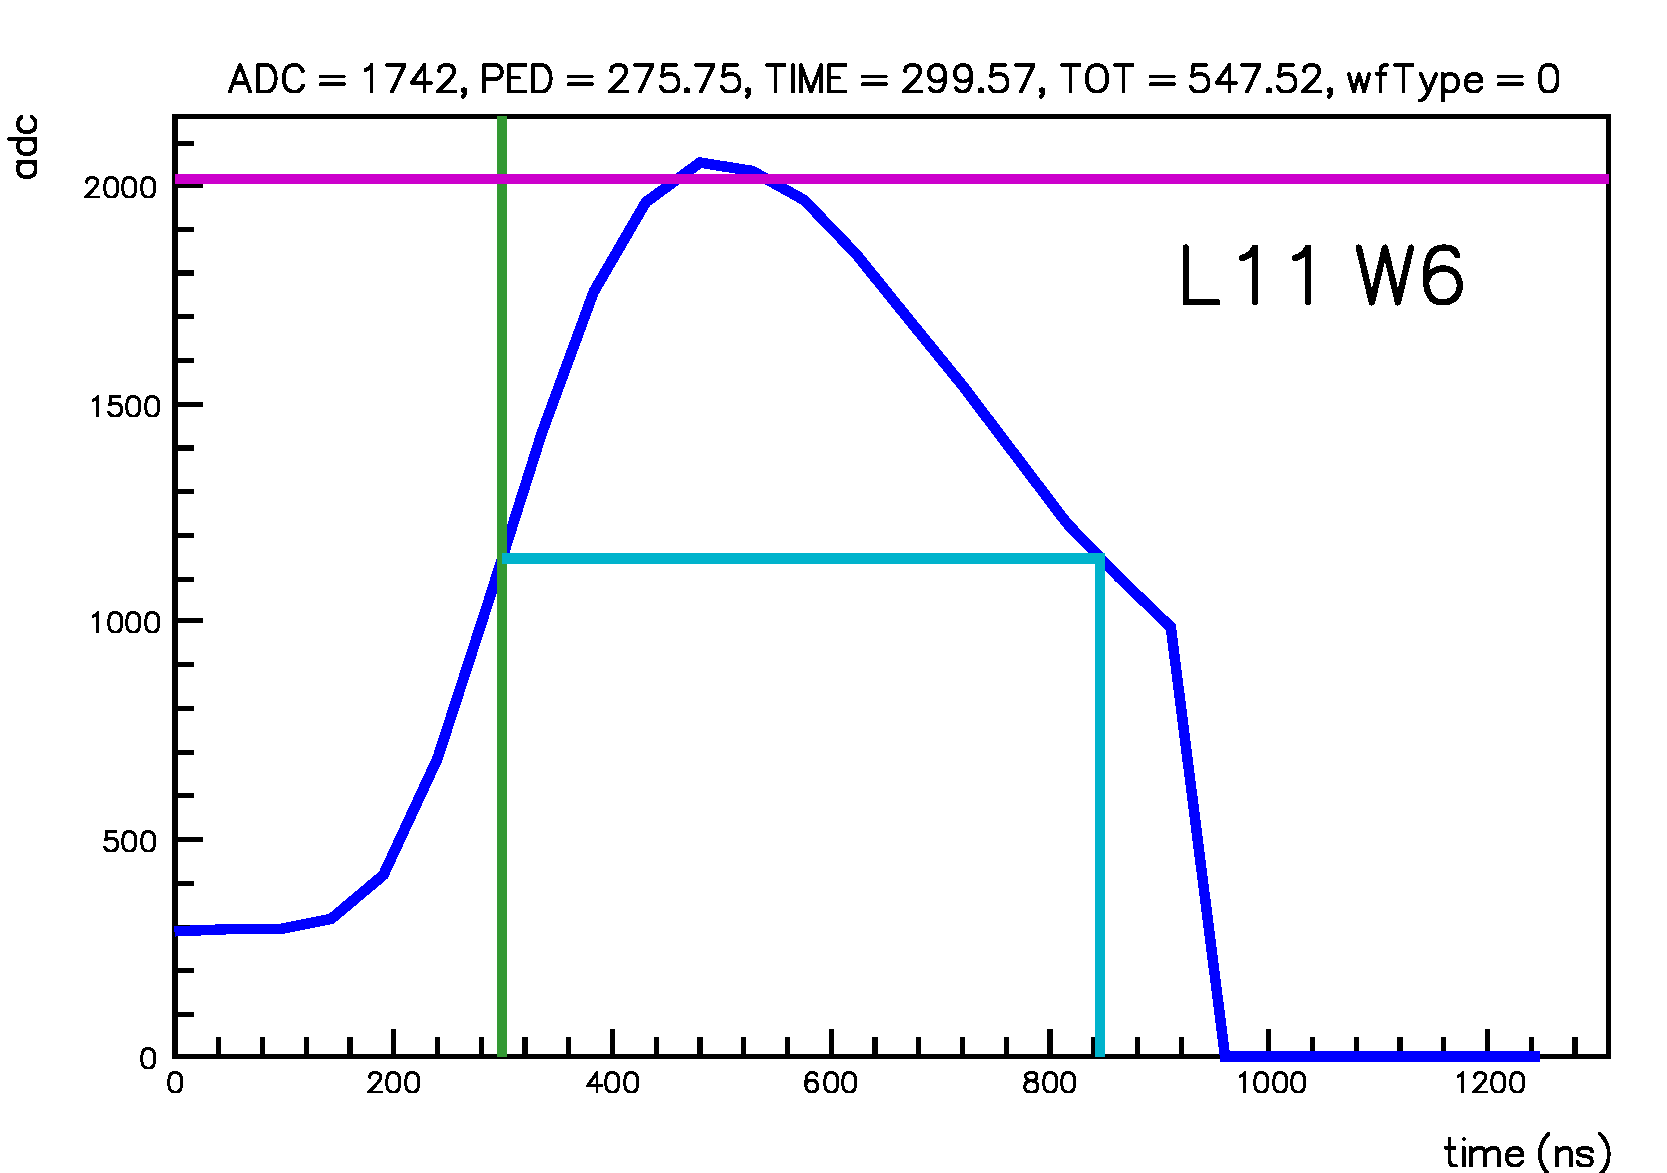
\includegraphics[width=0.24\linewidth]{figures/wf0_normal.pdf} &
        \end{tabular}
    }
    
\end{frame}


\begin{frame}{From hit selection to track fitting}
    \begin{itemize}
        \item Selection criteria (wfType $\leq$ 2 and time cuts)
        \item The occupancy in the AHDC is much lower after the hit selection
        \item It simplifies the task of the track finder
        \item The remaining hits are clustered into track candidates
        \item The track candidates are fitted
        \item The tracking is combined with the ATOF to recover the position and the momentum at the interaction point
    \end{itemize}

    \vspace{0.3cm}
    \centering

    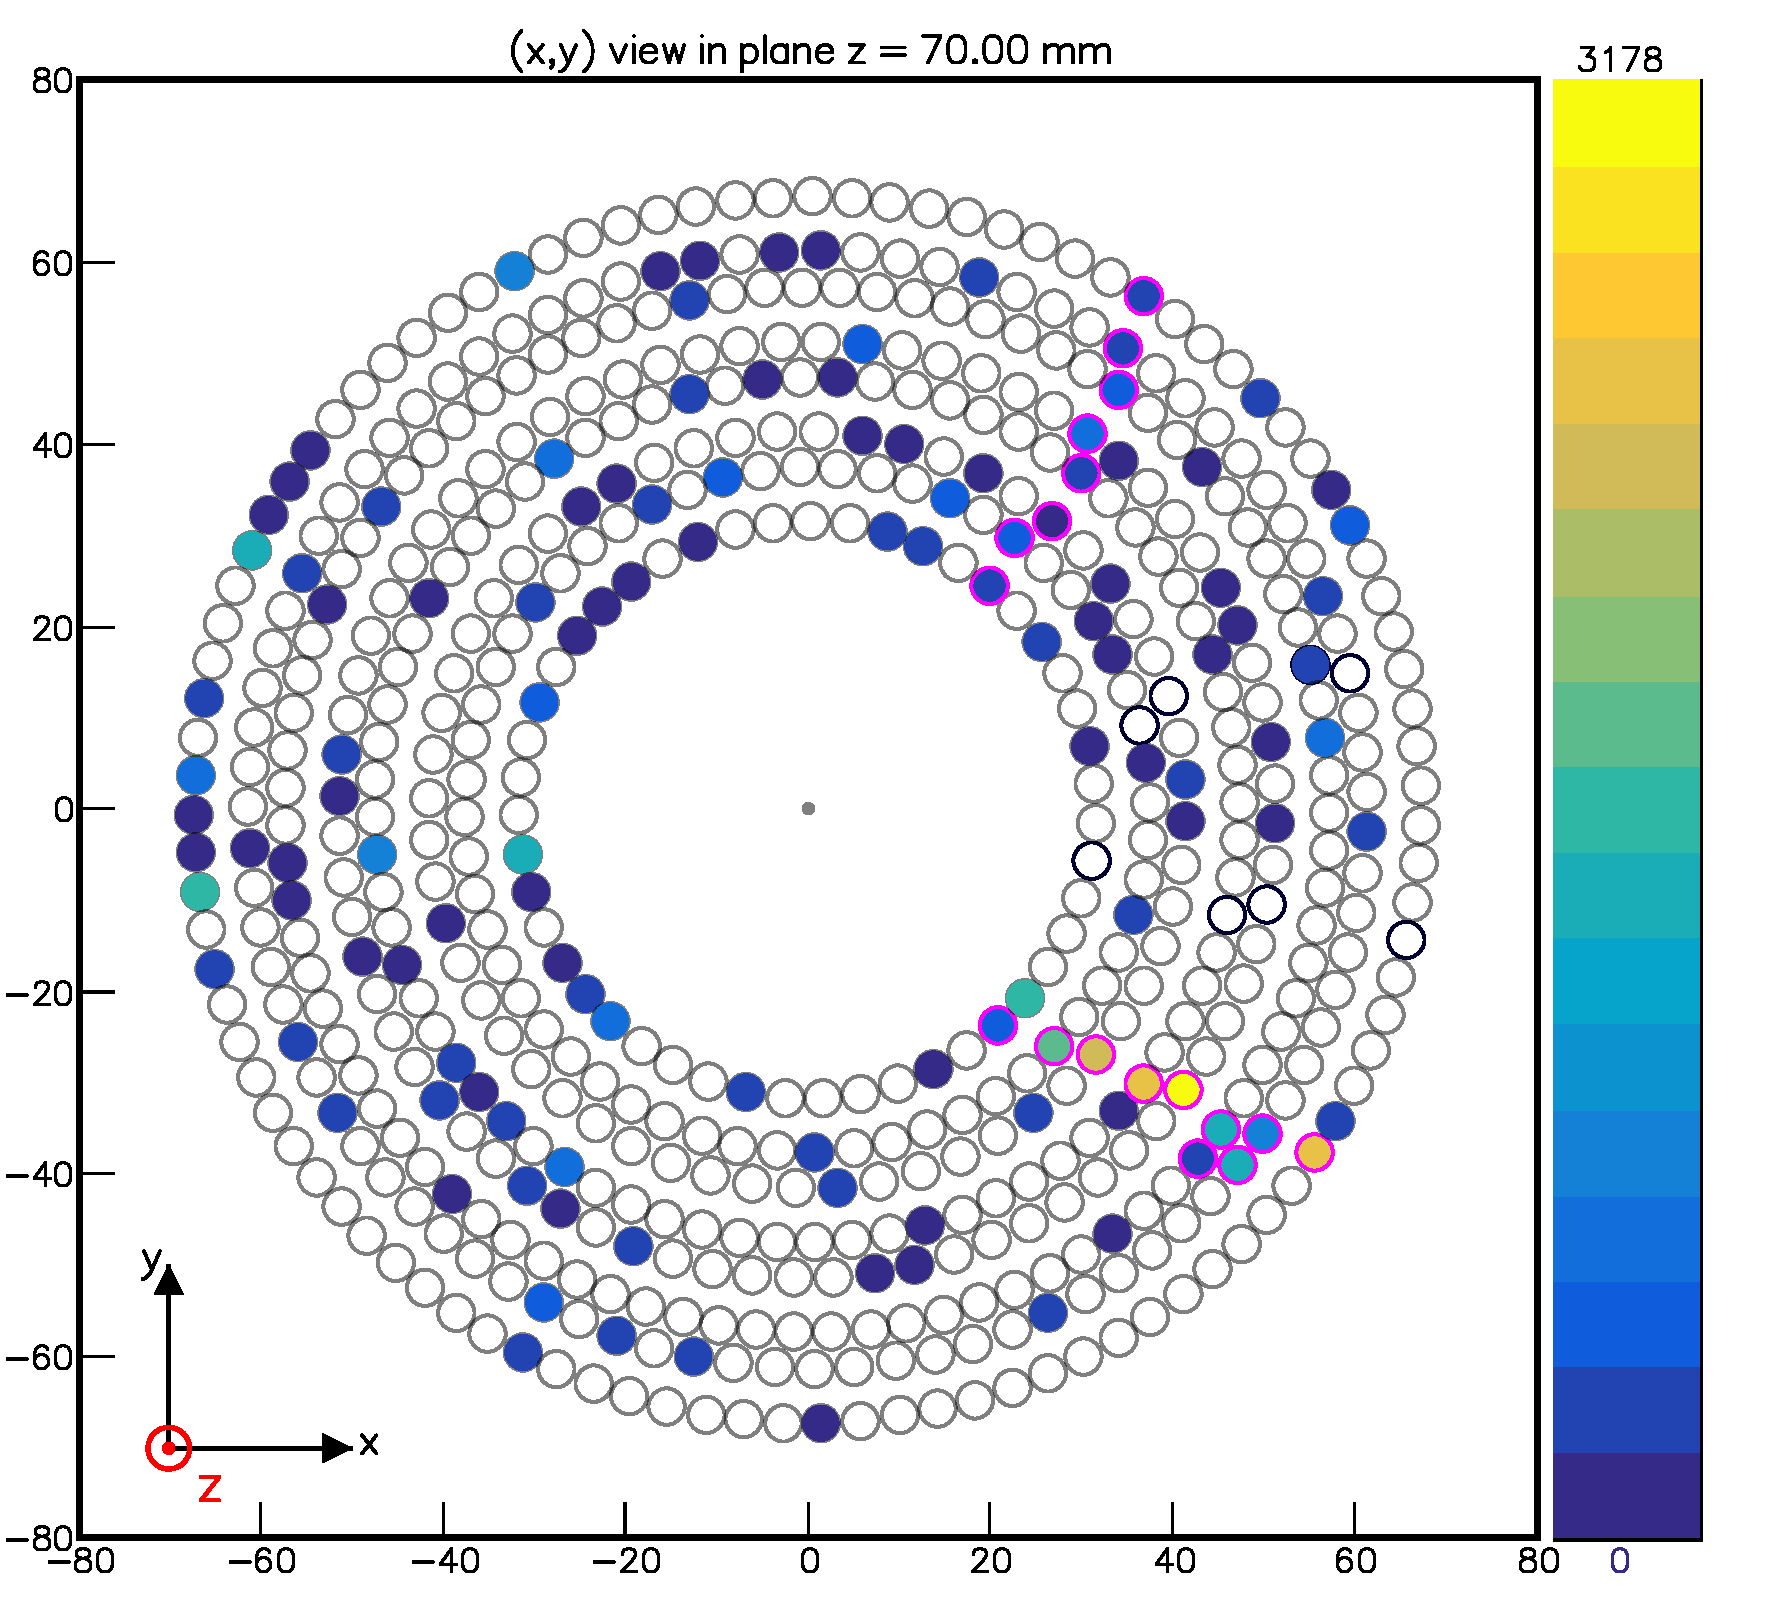
\includegraphics[width=0.38\linewidth]{figures/EventDisplay_for_waveformPerLayer.pdf}
    \hspace{0.1cm}
    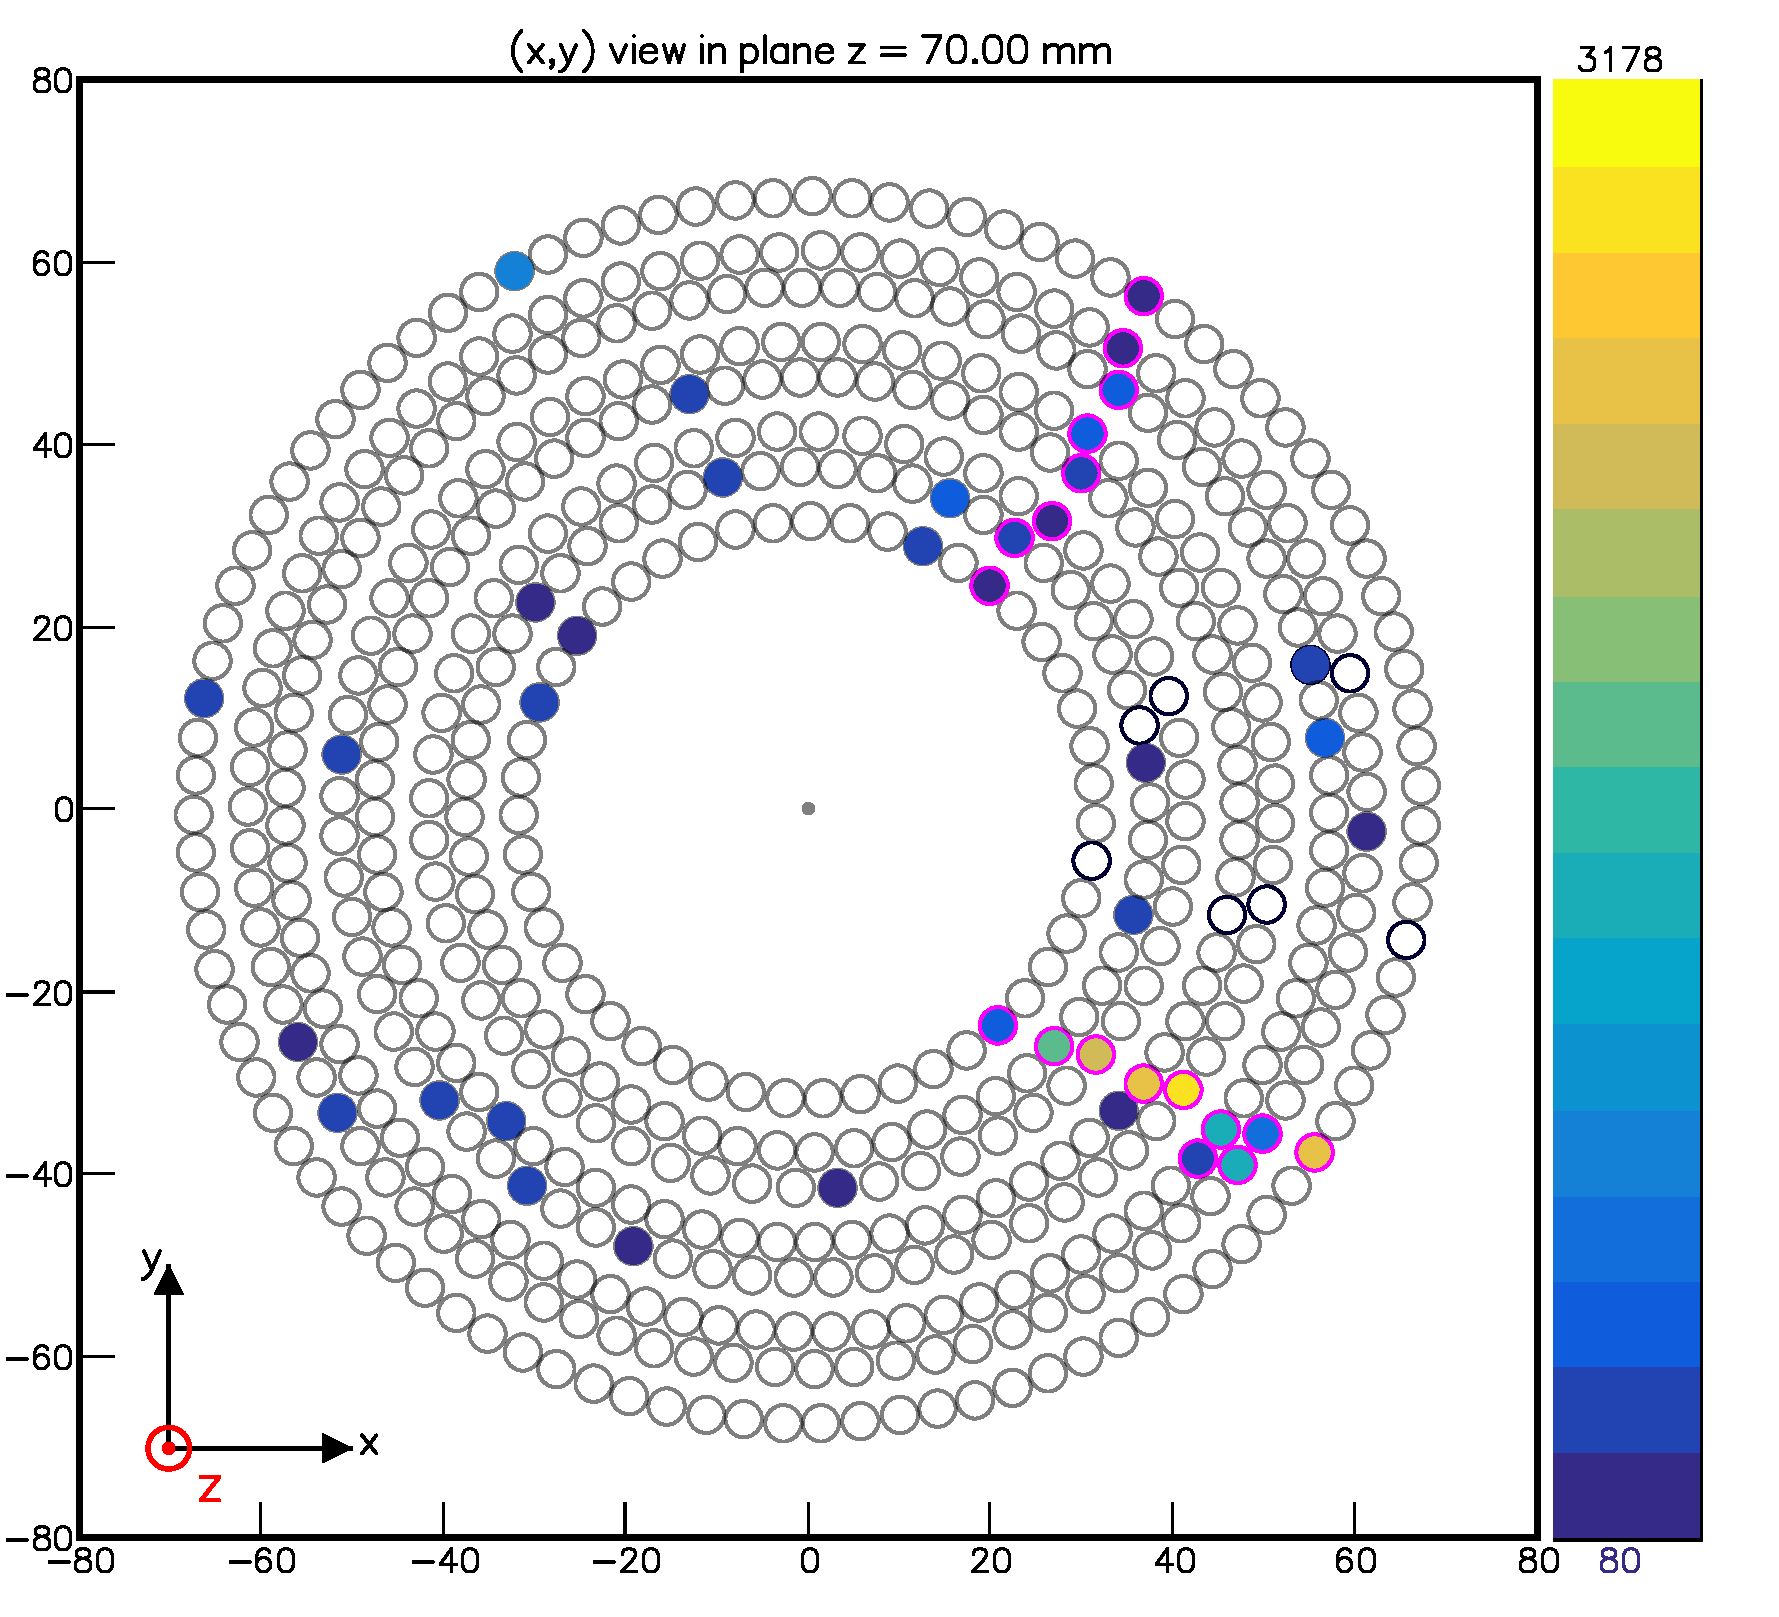
\includegraphics[width=0.38\linewidth]{figures/EventDisplay_for_waveformPerLayer_after_cuts.pdf}
    
\end{frame}


\begin{frame}{Time-to-distance calibration}
    \begin{itemize}
        \item It converts the reconstructed time into distance
        \item From the first time-to-distance to the current one
        %\item 
            % \begin{itemize}
            %     \item Layer by layer
            % \end{itemize}
        %\item Work on the automatization of the time to distance (layer by layer)
    \end{itemize}

    
    \vspace{0.3cm}
    %\centering

    \begin{minipage}{0.54\linewidth}

        
\includegraphics[height=2.5cm,width=3.2cm]{figures/time2distance.pdf}
        
\includegraphics[height=2.5cm,width=3.2cm]{figures/residual_post_time2distance_calib.pdf}

        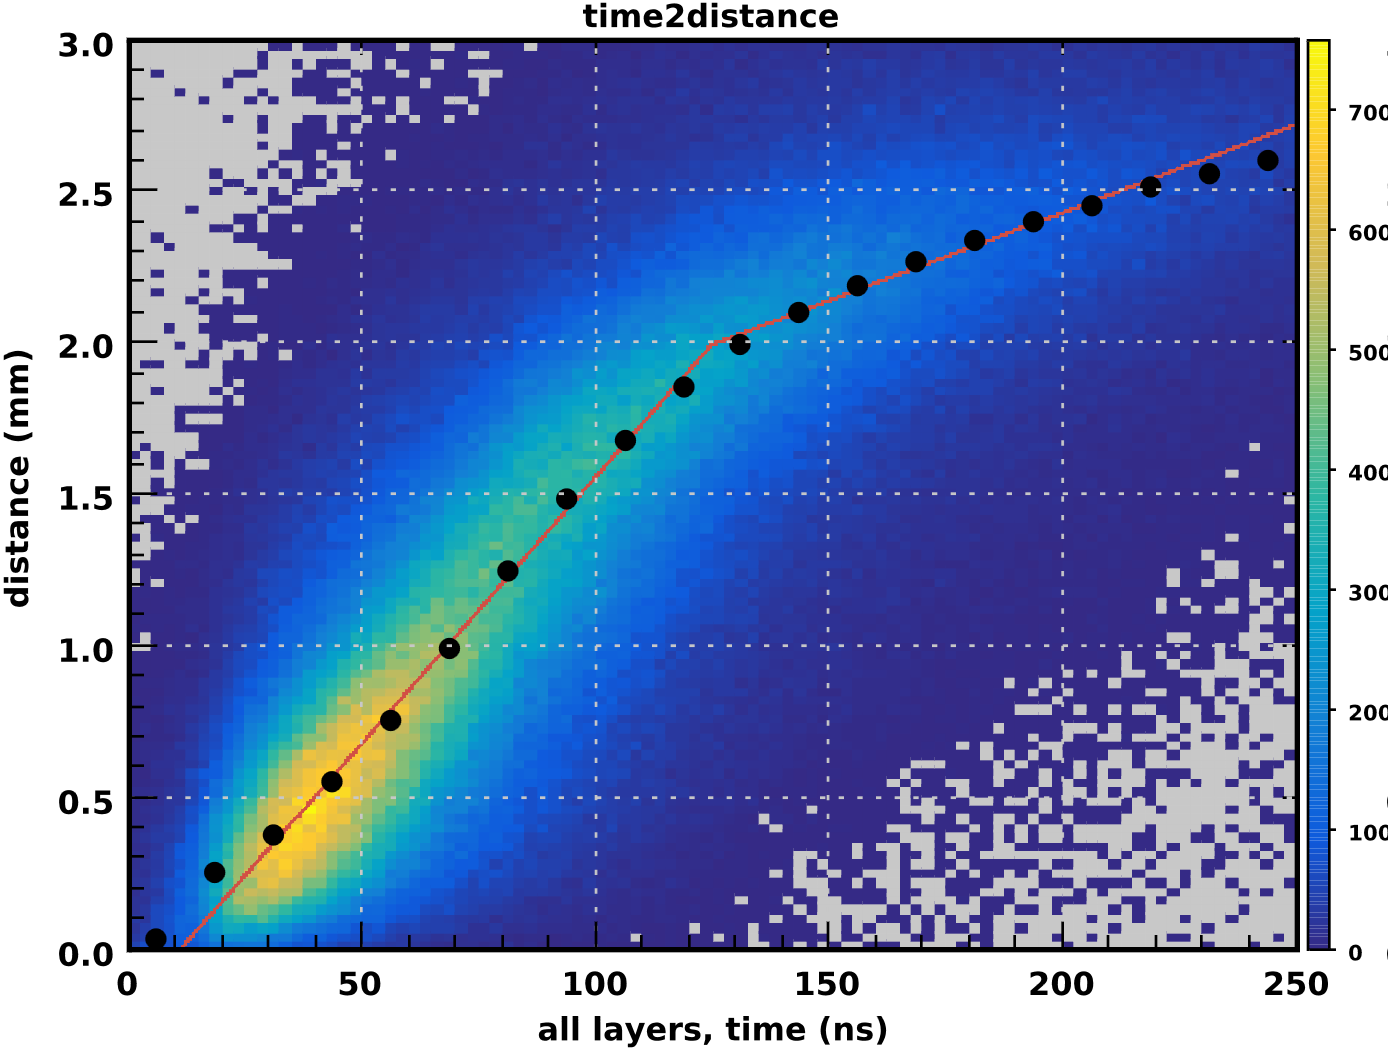
\includegraphics[height=2.5cm,width=3.2cm]{figures/new_t2d.png}
        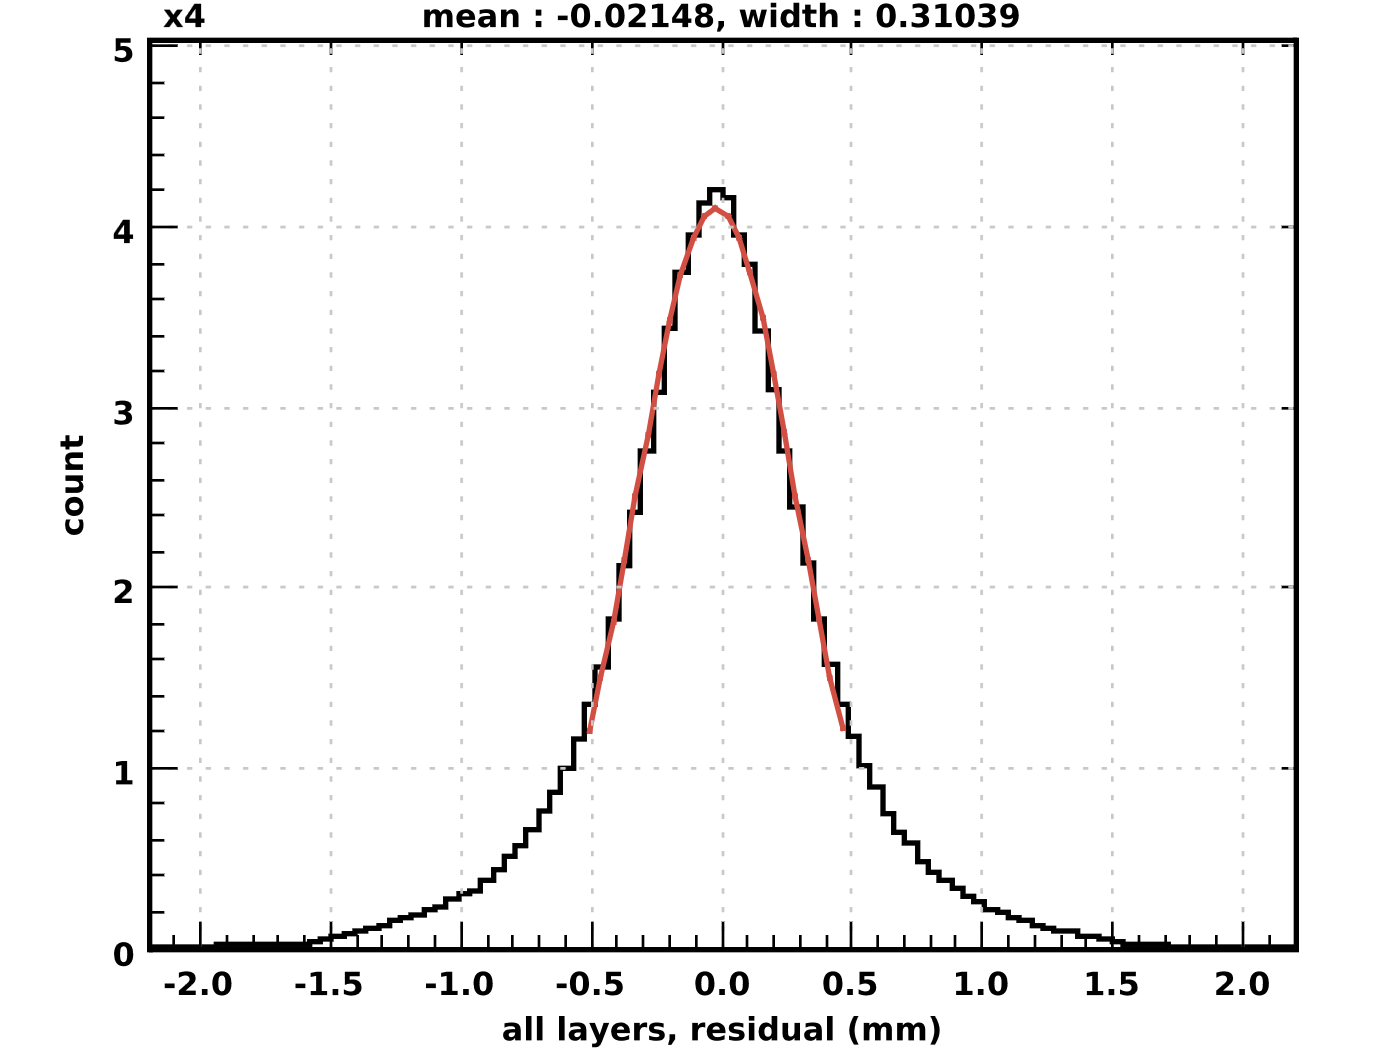
\includegraphics[height=2.5cm,width=3.2cm]{figures/residual_from_new_t2d.png}
    \end{minipage}
    \begin{minipage}{0.45\linewidth}
        
\includegraphics[width=\linewidth]{figures/build/residual_illustration.pdf}
    \end{minipage}
    
\end{frame}


\begin{frame}{Alignment}
    \begin{itemize}
        \item Alignment
    \end{itemize}
    
\end{frame}


\begin{frame}{Simulation}
    \begin{itemize}
        \item 
    \end{itemize}
    
\end{frame}


\begin{frame}{Issues fixed -- Wire swaps}
    \begin{itemize}
        \item 
    \end{itemize}
    
\end{frame}


\begin{frame}{Plan for the final year}
    \begin{itemize}
        \item 
    \end{itemize}
\end{frame}










\end{document}


